
%(BEGIN_QUESTION)
% Copyright 2011, Tony R. Kuphaldt, released under the Creative Commons Attribution License (v 1.0)
% This means you may do almost anything with this work of mine, so long as you give me proper credit

An operator reports a series of false pressure alarms reported by pressure indicating recorder PIR-139 every few minutes.  An instrument technician investigated this problem the previous day and declared it was most likely due to an electrical wiring fault between PT-139 and PIR-139 after measuring some intermittent high-current signals at the input terminals of PIR-139:

$$\includegraphics[width=15.5cm]{i0005rx01.eps}$$

You are called to re-examine this system, because the other instrument technician didn't actually do anything to fix the problem.  Your first test is to close the block (isolation) valve between PT-139 and the process pipe.  After doing this, the mysterious pressure alarms cease.  Later, you re-open that block valve and the pressure alarms resume.

\vskip 10pt

Explain what the results of this simple test tell you about the nature and location of the fault.  Does it confirm the first technician's diagnosis, or does it point to something else being wrong?  Explain your answer in detail.

\vskip 20pt \vbox{\hrule \hbox{\strut \vrule{} {\bf Suggestions for Socratic discussion} \vrule} \hrule}

\begin{itemize}
\item{} One detail not described in the scenario is just how the first technician measured those intermittent high-current signals at PIR-139.  Presumably it could have been done by continuously monitoring the display of a digital multimeter (DMM) long enough to see an alarm event occur.  However, if the alarm events were infrequent enough, this could be a laborious task for someone to continuously watch a meter waiting to see the current change.  Describe how you could use the {\it Min/Max} mode of a DMM instead to ``automate'' this task and free up the technician's time.
\end{itemize}

\underbar{file i02553}
%(END_QUESTION)





%(BEGIN_ANSWER)


%(END_ANSWER)





%(BEGIN_NOTES)

The fact that the alarms disappeared when the transmitter was isolated from process fluid pressure tells us that the transmitter is actually seeing fluid pressure transients, and that the problem is {\it not electrical in nature}.

%INDEX% Measurement, pressure: troubleshooting
%INDEX% Process: oily water sump (realistic P&ID shown)

%(END_NOTES)

